\pdfoutput=1
% =====================================================================
% arXiv preprint (non-anonymous). Primary category: cs.LG (cross-list cs.IR)
% Every number is a macro from figures/numbers.tex, generated by
% make_tables.py from experiments/arxiv_v2_rederive/results/*.json.
% Build:  pdflatex main.tex && bibtex main && pdflatex main.tex x2
% =====================================================================
\documentclass[sigconf,nonacm]{acmart}
\usepackage{bm}
\usepackage{cleveref}
\usepackage{xspace}
\usepackage{float}
\usepackage{placeins}
\usepackage{enumitem}
\usepackage{booktabs}
% AUTO-GENERATED by make_tables.py -- do not edit
\newcommand{\nnTest}{2,538,132}
\newcommand{\nnTrain}{8,248,933}
\newcommand{\nnLabels}{24}
\newcommand{\nnVal}{761,439}
\newcommand{\nwMax}{8,248,932}
\newcommand{\nwMin}{78}
\newcommand{\npopMAP}{0.535}
\newcommand{\nSraw}{0.120}
\newcommand{\nSplIsoId}{0.501}
\newcommand{\nSplIsoPrior}{0.784}
\newcommand{\nSplIsoExcl}{0.784}
\newcommand{\nSpooled}{0.260}
\newcommand{\nSceil}{0.786}
\newcommand{\nSauc}{0.785}
\newcommand{\nSsatOne}{16.0}
\newcommand{\nSsatZero}{34.9}
\newcommand{\nSnDead}{3}
\newcommand{\nWraw}{0.776}
\newcommand{\nWplIsoId}{0.434}
\newcommand{\nWplIsoPrior}{0.828}
\newcommand{\nWplIsoExcl}{0.830}
\newcommand{\nWpooled}{0.776}
\newcommand{\nWceil}{0.831}
\newcommand{\nWauc}{0.920}
\newcommand{\nWsatOne}{0.0}
\newcommand{\nWsatZero}{0.0}
\newcommand{\nWnDead}{3}
\newcommand{\nNraw}{0.806}
\newcommand{\nNplIsoId}{0.817}
\newcommand{\nNplIsoPrior}{0.820}
\newcommand{\nNplIsoExcl}{0.822}
\newcommand{\nNpooled}{0.807}
\newcommand{\nNceil}{0.824}
\newcommand{\nNauc}{0.852}
\newcommand{\nNsatOne}{0.0}
\newcommand{\nNsatZero}{24.7}
\newcommand{\nNnDead}{3}
\newcommand{\nSplIsoIdRel}{+316.8}
\newcommand{\nSplIsoPriorRel}{+552.2}
\newcommand{\nWplIsoIdRel}{-44.1}
\newcommand{\nWplIsoPriorRel}{+6.7}
\newcommand{\nNplIsoPriorRel}{+1.7}
\newcommand{\nSelkan}{0.155}
\newcommand{\nSloss}{0.686}
\newcommand{\ntieShare}{3}
\newcommand{\nrepairShare}{97}
\newcommand{\nceilShare}{97}
\newcommand{\nelkanShare}{5}
\newcommand{\nSceilGap}{0.020}
\newcommand{\nSplIsoPriorCeilGap}{0.003}
\newcommand{\nnCappedShift}{14}
\newcommand{\nSplOffsetPrior}{0.737}
\newcommand{\nWplOffsetPrior}{0.689}
\newcommand{\nNplOffsetPrior}{0.817}
\newcommand{\noffsetShare}{90}
\newcommand{\nSplPlattPrior}{0.767}
\newcommand{\nWplPlattPrior}{0.775}
\newcommand{\nNplPlattPrior}{0.812}
\newcommand{\nplattShare}{94}
\newcommand{\nSplBetaPrior}{0.776}
\newcommand{\nWplBetaPrior}{0.775}
\newcommand{\nNplBetaPrior}{0.818}
\newcommand{\nbetaShare}{96}
\newcommand{\nlabelFreeShare}{88}
\newcommand{\nSplIsoPriorFour}{0.7836}
\newcommand{\nSceilFour}{0.7862}
\newcommand{\nWplPlattIsoGap}{0.053}
\newcommand{\nNplPlattIsoGap}{0.009}
\newcommand{\nNplBetaIsoGap}{0.003}
\newcommand{\nWdeadMeanInTop}{3.00}
\newcommand{\nWdeadAllRowsPct}{100}
\newcommand{\nWdeadRawMean}{0.120}
\newcommand{\nWaliveCalMax}{0.0106}
\newcommand{\nSlabelFree}{0.723}
\newcommand{\nwhatifN}{0.806}
\newcommand{\nwhatifIdeal}{0.667}
\newcommand{\nwhatifHalf}{0.760}
\newcommand{\nwhatifS}{0.120}
\newcommand{\noddsShare}{20}
\newcommand{\nsatShare}{80}
\newcommand{\noverlapWhatif}{3.85}
\newcommand{\noverlapS}{2.68}
\newcommand{\nfracRowsChangedWhatif}{98}
\newcommand{\nidealRel}{-17.3}
\newcommand{\nSactualRel}{-85.1}
\newcommand{\nrepairExtraShare}{76}
\newcommand{\nbootB}{2000}
\newcommand{\nbootN}{51,403}
\newcommand{\nciSpriorMinusPop}{+0.248~[+0.245,\,+0.251]}
\newcommand{\nciSidMinusPop}{-0.035~[-0.038,\,-0.031]}
\newcommand{\nciWprior}{+0.052~[+0.050,\,+0.054]}
\newcommand{\nciNprior}{+0.014~[+0.013,\,+0.015]}
\newcommand{\nciNminusS}{+0.023~[+0.021,\,+0.024]}
\newcommand{\nnMulan}{8}
\newcommand{\nnLearners}{5}
\newcommand{\nenronStrongRawWone}{0.653}
\newcommand{\nenronStrongRawWr}{0.592}
\newcommand{\nenronStrongInvWr}{0.656}
\newcommand{\nenronStrongWhatifWr}{0.450}
\newcommand{\nmedStrongDistinctWone}{24}
\newcommand{\nmedStrongDistinctWtenr}{2.7}
\newcommand{\nmedStrongCeilWone}{0.603}
\newcommand{\nmedStrongCeilWtenr}{0.463}
\newcommand{\nmedL}{45}
\newcommand{\nmedDeadCal}{21}
\newcommand{\nmedIdVsPriorMaxGap}{0.18}
\newcommand{\nnMulanModest}{4}
\newcommand{\nbirdsNcal}{96}
\newcommand{\nbirdsRawWone}{0.593}
\newcommand{\nbirdsPlIsoPriorWone}{0.549}
\newcommand{\nmedNcal}{99}
\newcommand{\nmedRawWone}{0.683}
\newcommand{\nmedPlIsoPriorWone}{0.651}
\newcommand{\ngenbaseDistinctWone}{69}
\newcommand{\ngenbaseDistinctWr}{51}
\newcommand{\nmedLogregRawWone}{0.797}
\newcommand{\nmedLogregRawWr}{0.806}
\newcommand{\nmedXgbRawWone}{0.464}
\newcommand{\nmedXgbRawWr}{0.522}
\newcommand{\nnHurtAllLearners}{1}
\newcommand{\nhurtDatasets}{birds, emotions, enron, flags, genbase, medical, scene}
\newcommand{\nhurtDefaultDatasets}{birds, flags, medical}
\newcommand{\nnHurtDefault}{3}
\newcommand{\nmaxAbsDeltaElsewhere}{0.01}
\newcommand{\ncalPosMedEmotions}{32}
\newcommand{\ncalPosMedScene}{60}
\newcommand{\ncalPosMedFlags}{22}
\newcommand{\ncalPosMedBirds}{5}
\newcommand{\ncalPosMedYeast}{126}
\newcommand{\ncalPosMedGenbase}{5}
\newcommand{\ncalPosMedEnron}{6}
\newcommand{\ncalPosMedMedical}{1}
\newcommand{\nnWhatifClose}{7}
\newcommand{\nmaxDropModest}{0.041}
\newcommand{\nenronDefaultWhatifWr}{0.596}
\newcommand{\nenronDefaultRawWr}{0.614}
\newcommand{\ngenbaseDefaultWhatifWr}{0.927}
\newcommand{\ngenbaseDefaultRawWr}{0.868}
\newcommand{\nsynL}{20}
\newcommand{\nsynN}{20,000}
\newcommand{\nsynSeeds}{3}
\newcommand{\nsynK}{5}
\newcommand{\nsynTrueD}{0.576}
\newcommand{\nsynLRrawD}{0.302}
\newcommand{\nsynLRinvD}{0.575}
\newcommand{\nsynLRrawDeZero}{0.575}
\newcommand{\nsynSmallInvD}{0.198}
\newcommand{\nsynSmallCeilD}{0.565}
\newcommand{\nleafLgbmMaxSat}{8}
\newcommand{\nleafMedCeilFiftyWone}{0.610}
\newcommand{\nleafMedCeilFiftyWhundred}{0.491}


\clubpenalty=10000
\widowpenalty=10000
\displaywidowpenalty=10000
\brokenpenalty=10000
\emergencystretch=2em
\pdfinfo{ /Author (Akifumi Goto) /Keywords (class imbalance; class weights; multi-label classification; top-K recommendation; probability calibration; isotonic regression; gradient boosting) }

\newtheorem{proposition}{Proposition}
\newtheorem{lemma}{Lemma}
\newtheorem{corollary}{Corollary}
\crefname{proposition}{Proposition}{Propositions}
\Crefname{proposition}{Proposition}{Propositions}
\crefname{lemma}{Lemma}{Lemmas}
\Crefname{lemma}{Lemma}{Lemmas}
\crefname{corollary}{Corollary}{Corollaries}
\Crefname{corollary}{Corollary}{Corollaries}
\crefname{section}{Section}{Sections}
\Crefname{section}{Section}{Sections}
\crefname{table}{Table}{Tables}
\Crefname{table}{Table}{Tables}
\crefname{figure}{Figure}{Figures}
\Crefname{figure}{Figure}{Figures}
\renewcommand{\qedsymbol}{}

\newcommand{\Sm}{\textsf{LGBM-w}\xspace}
\newcommand{\Wm}{\textsf{WGB}\xspace}
\newcommand{\Nm}{\textsf{LGBM-0}\xspace}
\newcommand{\mapk}{\mathrm{MAP}@K\xspace}
\newcommand{\mapseven}{\mathrm{MAP}@7\xspace}

\setcopyright{none}
\settopmatter{printacmref=false}
\renewcommand\footnotetextcopyrightpermission[1]{}
\pagestyle{plain}

\begin{document}

\title{Don't Reweight, Calibrate: Per-Label Class Weights Distort Top-$K$ Ranking, the Textbook Inversion Does Not Repair It, and Per-Label Calibration Does}

\author{Akifumi Goto}
\email{souldrive7@gmail.com}
\affiliation{\institution{Independent researcher}\country{Japan}}

\begin{abstract}
Practitioners who rank $L$ labels per row (a customer's next product, a document's tags) routinely train one-vs-rest models with a label-specific positive-class weight such as \texttt{scale\_pos\_weight}$=n_{-}/n_{+}$ to counter imbalance. The textbook account of what this does is Elkan's identity: a positive weight $w_j$ shifts label $j$'s log-odds by $\ln w_j$, so within a row the model ranks by $w_j\cdot\mathrm{odds}(p_{ij})$ instead of by the marginal $p_{ij}$ that is Bayes-optimal for precision@$K$, and the shift can be undone analytically. We show on the Santander product-recommendation benchmark (\nnTest{} test rows, \nnLabels{} labels) that this account explains only a fifth of the damage. LightGBM one-vs-rest scores $\mapseven=\nNraw$ unweighted and $\nSraw$ with the recommended weights; the ideal odds shift applied to the unweighted model gives $\nwhatifIdeal$ (\noddsShare\% of the loss), and the analytic inversion of the trained weighted model recovers almost nothing ($\nSelkan$). The rest of the distortion is not the shift $\ln w_j$ that the identity prescribes: weights up to \nwMax{} push every positive-containing leaf to a fitted rate of one (we give the leaf-level condition), \nSsatOne\% of test cells sit at exactly $1.0$, and the realized shift is a different constant for most labels with a non-linear remainder. It is still per-label monotone, so per-label calibration repairs it: an intercept-only logit shift fitted per label recovers \noffsetShare\% of the loss, per-label Platt scaling \nplattShare\%, and isotonic regression with a prior fallback for labels without calibration positives \nrepairShare\% ($\nSplIsoPriorFour$ against an in-sample per-label isotonic ceiling of $\nSceilFour$); the remaining \ntieShare\% lies above that ceiling, and the cells tied at exactly $1.0$ or $0.0$ are its visible cause. The fallback is decisive: the identity fallback collapses a direct-probability model from $\nWraw$ to $\nWplIsoId$ and leaves the weighted model below the popularity baseline, whereas the prior fallback improves all three base models; a shared (pooled) map never inverts a pair and therefore cannot repair the weighted model beyond tie resolution. Dose-response experiments on \nnMulan{} MULAN benchmarks with \nnLearners{} learners (LightGBM, XGBoost, logistic regression, and an MLP with BCE \texttt{pos\_weight}) and a synthetic study with known marginals reproduce the odds shift, its exact inversion under a realizable learner, and the failure of the inversion under capacity limits, and also show that per-label calibration hurts when labels have few calibration positives. The recommendation is simple: estimate marginals with an unweighted proper loss, calibrate per label with a prior fallback for every label whose calibration positives cannot support its map, and decide at top-$K$.
\end{abstract}

\maketitle

\section{Introduction}
\label{sec:intro}

Ranking many binary labels within a row is the operational core of product recommendation, tagging, and risk triage: for each customer the system scores every product, sorts, and shows the top $K$~\cite{Jain2016XMLLoss,Menon2019Reductions}. The labels are almost always imbalanced, and the most common remedy in gradient-boosting practice is a per-label positive-class weight, \texttt{scale\_pos\_weight} in XGBoost and LightGBM~\cite{Chen2016XGBoost,Ke2017LightGBM}, for which the XGBoost documentation suggests the value $n_-/n_+$~\cite{XGBoostDocs}. The same recipe appears as \texttt{pos\_weight} in binary cross-entropy for neural multi-label models.

This paper shows that label-specific weights are not a free choice when the deliverable is a per-row ranking, that most of the damage they do is not the part textbook theory describes, and that the right repair is per-label calibration with a carefully chosen fallback rather than the textbook inversion. Two facts are classical. Ranking labels by their marginal probability $p_{ij}=\Pr(y_{ij}=1\mid x_i)$ is Bayes-optimal for precision@$K$, and the one-vs-rest reduction with a proper loss is consistent for it~\cite{Dembczynski2012Univariate,Menon2019Reductions,Wydmuch2018PLT}. A positive-class weight $w$ moves the population minimizer of a proper loss from $p$ to $wp/(wp+1-p)$, an odds shift by $w$~\cite{Elkan2001,Saerens2002}. Put together, a label-specific $w_j$ makes the model rank by $w_j\cdot\mathrm{odds}(p_{ij})$, which is a different ranking whenever the weights differ. The XGBoost documentation itself warns that a re-balanced model no longer predicts the right probability~\cite{XGBoostDocs}. What we quantify here is (i) how much top-$K$ quality label-specific weights cost in multi-label practice, (ii) that only the odds-shift part of the loss can be predicted before training, and (iii) what finite-capacity learners do when $w_j$ is in the thousands or millions, as the documentation-recommended value is for rare labels, and which post-hoc repair then works.

\Cref{fig:one} summarizes the answer on the Santander product-recommendation benchmark (\nnTest{} test rows, \nnLabels{} products). LightGBM one-vs-rest with the same learning rate and leaf count reaches $\mapseven=\nNraw$ without weights and $\nSraw$ with $w_j=n_-/n_+$. Applying the ideal odds shift to the unweighted model's logits, which is exactly what Elkan's identity predicts for a weighted model that realizes the shift, gives $\nwhatifIdeal$: the textbook mechanism explains \noddsShare\% of the loss, and the analytic inversion of the trained weighted model recovers only \nelkanShare\% of it ($\nSelkan$). The trained model's distortion is not the prescribed shift. With $w_j$ up to \nwMax{}, every leaf that contains a single positive is pushed to a fitted rate of one (\cref{lem:leaf}) and \nSsatOne\% of all test cells sit at exactly $1.0$; the realized per-label shift is a different constant for most labels (an intercept-only shift fitted on a calibration split recovers \noffsetShare\% of the loss) with a non-linear remainder (per-label isotonic regression recovers \nrepairShare\%). Three facts then decide what can be repaired. The distortion is still monotone within each label, so a per-label monotone map can undo it: isotonic regression with a prior fallback returns $\nSplIsoPrior$, within $\nSplIsoPriorCeilGap$ of the in-sample per-label isotonic ceiling ($\nSceil$). The remaining $\nSceilGap$, \ntieShare\% of the loss, lies above that ceiling; the cells tied at exactly $1.0$ or $0.0$ are its visible cause. And a shared map cannot help beyond tie resolution, because it never inverts a pair (\cref{prop:sep}).

The second half of the paper concerns the fallback that makes or breaks per-label calibration. Per-label isotonic regression has been reported to break top-$k$ accuracy in multi-class settings~\cite{Patel2021IMax}, and the extreme multi-label literature deliberately uses one shared monotone map so that precision@$k$ is untouched~\cite{Ullah2025XMLCCalib}. We find that on this benchmark the sign of per-label calibration is decided by a single implementation detail: what the calibrator returns for a label whose calibration split has no positives. Falling back to the identity leaves those labels on the raw scale while every other label shrinks to its prevalence, so the dead labels occupy the top of every row; the direct-probability model \Wm drops from $\nWraw$ to $\nWplIsoId$, and the weighted model stays below the popularity baseline. Falling back to the prior removes the effect, and the same calibrator then improves all three base models to within $0.01$ of their oracle ceilings.

\paragraph{Contributions}
\begin{enumerate}[leftmargin=*,nosep]
\item \textbf{Where the textbook account stops.} Using Elkan's identity as a what-if device, we separate the loss of a weighted top-$K$ ranker on Santander into the ideal odds shift (\noddsShare\%), a further per-label monotone distortion that the analytic inversion with the known weights cannot undo but per-label calibration can (\nrepairExtraShare\%), and a remainder above the in-sample per-label isotonic ceiling (\ntieShare\%). The realized shift is a different constant for most labels (an intercept-only per-label shift recovers \noffsetShare\% of the loss) with a non-linear remainder. We give the leaf-level saturation condition behind this (\cref{lem:leaf}) and confirm the formula on single trees.
\item \textbf{The fallback decides the sign.} Per-label isotonic regression improves all three Santander base models when labels without calibration positives are mapped to their prior; when those labels keep their raw scores it collapses the direct-probability model and leaves the weighted model below the popularity baseline (\cref{prop:dead}). A shared map never inverts a pair and therefore never repairs beyond tie resolution (\cref{prop:sep}, stated for non-decreasing maps with ties).
\item \textbf{Dose-response across \nnMulan{} benchmarks, \nnLearners{} learners and a synthetic study.} The odds shift is learner-agnostic and exactly invertible for a realizable learner; the inversion fails once the learner saturates; per-label calibration with a prior fallback recovers most of the loss where labels have enough calibration positives and hurts where they do not.
\item \textbf{A recipe.} Unweighted proper loss; per-label calibration with the prior as fallback for every label whose calibration split cannot support its map; decision at top-$K$; a common weight if optimization needs one; utilities multiplied into calibrated marginals if a weighted ranking is wanted.
\end{enumerate}
All numbers in this paper are generated by a single script from artifacts that will be released with the paper; the dead-label policy of every calibrator is explicit.

\section{Setup and Background}
\label{sec:setup}

Rows $i=1,\dots,n$ carry a feature vector $x_i$ and binary labels $y_{ij}\in\{0,1\}$ for $j=1,\dots,L$. The marginal is $p_{ij}=\Pr(y_{ij}=1\mid x_i)$ and $\pi_j=\Pr(y_{ij}=1)$ is the prevalence. A scorer $s$ produces $s_{ij}$; the system returns the $K$ labels with the largest $s_{ij}$ in row $i$. We evaluate with $\mapk$ in the Kaggle definition (average precision at $K$ per row, averaged over rows that have at least one positive) and report per-row bootstrap intervals.

\paragraph{Ranking by marginals is Bayes-optimal.} For precision@$K$ the population-optimal ranking within a row sorts labels by $p_{ij}$, and the one-vs-rest reduction with a proper binary loss is consistent for it~\cite{Dembczynski2012Univariate,Koyejo2015Consistent,Menon2019Reductions}; the precision@$k$ regret of a plug-in ranker is bounded by its marginal estimation error~\cite{Wydmuch2018PLT}. Everything below is about scorers that are monotone transformations of marginal estimates and therefore about when such transformations preserve or destroy the within-row order.

\paragraph{Separable post-hoc maps.} A post-hoc calibrator is \emph{separable} if it applies a non-decreasing map $g_j$ to label $j$ independently of the other labels in the row: $\tilde s_{ij}=g_j(s_{ij})$. Per-label Platt, isotonic, temperature, and beta calibration are separable; so is the shared (pooled) isotonic map of~\cite{Ullah2025XMLCCalib}, with $g_j\equiv g$. Row-dependent maps such as intra-order-preserving functions~\cite{Rahimi2020IntraOrder} are not separable and are outside this paper's scope.

\paragraph{Weighted training.} A positive-class weight $w_j>0$ multiplies the loss of positive examples of label $j$. For LightGBM and XGBoost this is \texttt{scale\_pos\_weight}; for a neural model it is \texttt{pos\_weight} in \texttt{BCEWithLogitsLoss}; the XGBoost documentation suggests $w_j=n_{-,j}/n_{+,j}$~\cite{XGBoostDocs}.

\section{Theory: Two Mechanisms and What Calibration Can Fix}
\label{sec:theory}

\subsection{Separable maps preserve within-row order iff they are shared}

\begin{proposition}[Shared maps never invert, distinct maps can]
\label{prop:sep}
Let $g_1,\dots,g_L$ be non-decreasing maps on a common interval $I$. (a) If $g_1=\dots=g_L$, the separable calibrator never creates a strict inversion: $s_{ij}>s_{ik}$ implies $\tilde s_{ij}\ge\tilde s_{ik}$, with equality only when the two scores fall in the same plateau of the shared map. (b) If the maps are continuous and $g_j(a)\neq g_k(a)$ for some $a$ in the interior of $I$ and some $j\neq k$, there is a score vector whose strict within-row order is inverted.
\end{proposition}
\begin{proof}
(a) is monotonicity. (b) Say $g_j(a)<g_k(a)$. By continuity of $g_j$ there is $b>a$ in $I$ with $g_j(b)<g_k(a)$; the row with $s_{ij}=b>a=s_{ik}$ has $\tilde s_{ij}<\tilde s_{ik}$. If no such $b$ exists because $a$ is the right endpoint, use continuity of $g_k$ to pick $b<a$ with $g_k(b)>g_j(a)$ and the row $s_{ik}=b<a=s_{ij}$.
\end{proof}

The statement is folklore; shared class-wise binning~\cite{Patel2021IMax}, intra-order-preserving maps~\cite{Rahimi2020IntraOrder} and the shared map of~\cite{Ullah2025XMLCCalib} all rely on (a). We state it because both halves matter below. A shared map (pooled isotonic, global Platt or temperature) is \emph{rank-neutral} up to ties: it can never invert a pair, so it can never repair a within-row distortion, and the only way it changes a top-$K$ set is through plateaus, whose resolution depends on the tie rule of the sorter (this is visible in \cref{tab:ladder}). A per-label map can reorder, and in the population limit it \emph{should}: calibrated per-label maps return the marginals, and ranking by marginals is optimal. Per-label calibration therefore hurts only through estimation error, and the boundary case of estimation error is a label with no positives in the calibration split (\cref{sec:deadlabel}).

\subsection{Label-specific weights shift log-odds and change the ranking}

\begin{proposition}[Odds shift, after Elkan]
\label{prop:odds}
Let the population minimizer of a strictly proper binary loss with positive-class weight $w_j$ be $q_{ij}$. Then $\operatorname{logit}q_{ij}=\operatorname{logit}p_{ij}+\ln w_j$~\cite{Elkan2001,Saerens2002}. Consequently, for labels $j\neq k$ in row $i$ with $p_{ij}>p_{ik}$, the weighted scores reverse their order if and only if
\[
\operatorname{logit}p_{ij}-\operatorname{logit}p_{ik} \;<\; \ln w_k-\ln w_j .
\]
\end{proposition}
\begin{proof}
The weighted loss equals the unweighted loss under the tilted distribution in which positives are up-weighted by $w_j$, whose posterior odds are $w_j$ times the original odds; this is Elkan's identity. The flip condition is the difference of the two shifted logits.
\end{proof}

\begin{corollary}
\label{cor:odds}
(a) A common weight $w_j\equiv w$ never changes within-row order (it is a shared map in \cref{prop:sep}). (b) The set of flipped pairs, and hence the top-$K$ loss of the ideal weighted model, is a function of the unweighted logit gaps and the intended weights only; it can be computed from an unweighted model before weighted training (\emph{what-if}), up to that model's own estimation error, and it describes a weighted model that realizes the shift exactly, not necessarily the one a finite learner produces. (c) When $w_j p_{ij}\ll 1$, $q_{ij}\approx w_j p_{ij}$, so ranking by weighted scores approximates ranking by $w_j p_{ij}$, which is the optimal ranking for a propensity-weighted precision@$K$ with propensities $1/w_j$~\cite{Jain2016XMLLoss,Wydmuch2021PSPLT}: training-time weights silently change the metric being optimized. If a utility-weighted ranking is wanted, multiplying calibrated marginals by the utilities is exact, whereas training weights are approximate and, as the next lemma shows, harmful at large magnitude.
\end{corollary}

\subsection{Large weights saturate finite-capacity learners}

\begin{lemma}[Leaf saturation]
\label{lem:leaf}
For weighted log-loss the optimal constant prediction in a tree leaf with $n_+$ positives and $n_-$ negatives is the weighted rate $\rho(w)=wn_+/(wn_++n_-)$. Any leaf with $n_+\ge 1$ satisfies $\rho(w)\ge 1-n_-/(wn_+)$, so its prediction is within $\varepsilon$ of one as soon as $w\ge n_-/(\varepsilon n_+)$. All test cells routed to any such leaf receive predictions within $\varepsilon$ of one and lose their order across those leaves.
\end{lemma}
\begin{proof}
The weighted empirical log-loss of a constant $\rho$ in the leaf is $-wn_+\ln\rho-n_-\ln(1-\rho)$, minimized at $\rho=wn_+/(wn_++n_-)$. The bound follows from $1-\rho=n_-/(wn_++n_-)\le n_-/(wn_+)$.
\end{proof}

The lemma is exact for a single tree whose leaf values are weighted class frequencies (scikit-learn's \texttt{class\_weight}) and describes the fixed point that boosted ensembles approach when they fit the weighted objective well. Its practical content is a threshold: with the recommended $w_j=n_{-,j}/n_{+,j}\approx 1/\pi_j$ and leaves of at most $m$ negatives, every positive-containing leaf of a label with $\pi_j\le\varepsilon/m$ is within $\varepsilon$ of one. For Santander's rarest products ($w_j$ up to \nwMax) this is every leaf that has ever seen a positive. Two consequences follow, and they should be kept apart. First, the realized shift is no longer the constant $\ln w_j$ of \cref{prop:odds}, so the analytic inversion $q\mapsto q/(q+w(1-q))$ stops working; the distortion is still monotone within each label, so a per-label monotone map fitted on calibration data can undo it, and \cref{sec:santander} measures how much of it is a constant shift and how much is non-linear. Second, the cells that tie at one within a label have lost their mutual order, and no separable post-hoc map can recover it. The first effect is the large one in our data; the second is bounded by the gap between the in-sample per-label isotonic ceiling and the unweighted model. The tree analogue of a known fact is at work here: importance weights lose their effect once a flexible learner can fit the weighted objective~\cite{Byrd2019}, and a boosted tree with $w_j$ in the millions fits it by saturating.

\subsection{Uncalibratable labels and the fallback policy}
\label{sec:deadlabel}

A per-label calibrator fitted on a held-out split needs both classes. When a label has no positives in the split, scikit-learn's \texttt{IsotonicRegression} returns the constant zero and \texttt{LogisticRegression} raises; our own earlier one-vs-rest implementation, and any loop that catches the failure and passes the score through, returns the input unchanged. The choice matters:

\begin{proposition}[Identity fallback occupies the top]
\label{prop:dead}
Let label $d$ have no calibration positives and keep its raw score $s_{id}$, while every calibrated label $j$ is mapped by $g_j$ with $g_j(s)\le \bar q$ for all $s$ (isotonic outputs are bounded by the largest block mean of the calibration split). If $s_{id}>\bar q$ then $d$ is ranked above every calibrated label in row $i$ regardless of $y_{id}$; with $m$ such labels, $m$ of the top-$K$ slots are occupied by them.
\end{proposition}
The condition holds whenever raw scores are inflated relative to calibrated ones, which is exactly the situation that motivates calibration. A prior fallback ($\tilde s_{id}=\hat\pi_d$) or exclusion removes the effect. \Cref{sec:santander} shows that this single choice flips the sign of per-label calibration on the direct-probability model and decides whether the repaired weighted model beats the popularity baseline.

\section{Experiments}
\label{sec:exp}

\subsection{Santander: the same learner with and without weights}
\label{sec:santander}

\paragraph{Data and models.} The Santander Product Recommendation data~\cite{KaggleSantander2016} has \nnLabels{} products; we use the public time split with \nnTrain{} training rows and \nnTest{} test rows and the Kaggle $\mapseven$. Three base scorers produce test probabilities for every cell: \Nm, LightGBM one-vs-rest without weights (100 trees, learning rate $0.05$, 31 leaves); \Sm, LightGBM one-vs-rest with the same learning rate and leaf count but 60 trees and $w_j=n_{-,j}/n_{+,j}$ per label (between \nwMin{} and \nwMax); and \Wm, a Wasserstein gradient-boosting model with Beta-distributed outputs~\cite{Matsubara2024WGBoost} that estimates probabilities directly without weights. Post-hoc calibrators are fitted on a random 30\% of the test rows (seed 42, \nnVal{} rows) and evaluated on the remaining 70\%; \nSnDead{} labels have no positives in the calibration split. Per-row bootstrap intervals use $B=\nbootB$ resamples of the \nbootN{} evaluation rows that have at least one positive.

\begin{figure*}[t]
\centering
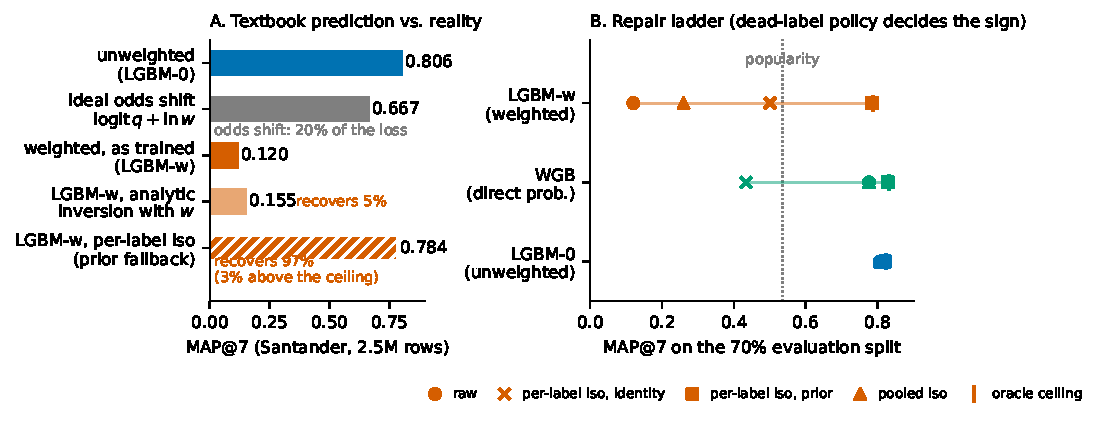
\includegraphics[width=\textwidth]{figures/fig1_decomposition_ladder.pdf}
\Description{Two panels of horizontal bar and dot charts of MAP at 7 on Santander. Panel A compares the unweighted model, the ideal odds-shifted model, the trained weighted model, its analytic inversion and its per-label isotonic repair. Panel B shows the repair ladder for three base models.}
\caption{\textbf{Per-label class weights cost far more than the odds shift predicts, per-label calibration repairs most of it, and the dead-label policy decides its sign.} \textbf{A.} $\mapseven$ of the unweighted LightGBM (\Nm), of the same model with the ideal odds shift $\ln w_j$ added to its logits (what \cref{prop:odds} predicts for a weighted model that realizes the shift), and of the weighted model actually trained (\Sm). The odds shift explains \noddsShare\% of the loss; per-label calibration recovers \nrepairShare\%; ties account for \ntieShare\%. \textbf{B.} Repair ladder for the three base models on the 70\% evaluation split: raw, per-label isotonic with identity or prior fallback for the \nSnDead{} labels without calibration positives, pooled isotonic, and the oracle per-label monotone ceiling (isotonic fitted in-sample on test labels); dotted line is ranking by training prevalence. Santander, \nnTest{} test rows, \nnLabels{} labels; 95\% bootstrap intervals are narrower than the markers (\cref{tab:ladder}).}
\label{fig:one}
\end{figure*}

\begin{table}[t]
\caption{Repair ladder on Santander ($\mapseven$, 70\% evaluation split, higher is better; the ceiling row is fitted and evaluated on all test rows, which differs from the split by less than $0.001$). The prior fallback turns per-label calibration from harmful to the best available repair on all three models; an intercept-only per-label shift already recovers most of the weighted model's loss; the shared map changes the weighted model only through ties; the weighted model's ceiling stays below the unweighted raw score. Saturation shares are exact-value counts over all test cells.}
\label{tab:ladder}
\footnotesize
\setlength{\tabcolsep}{4pt}
\begin{tabular}{@{}lccc@{}}
\toprule
 & \Sm & \Wm & \Nm \\
\midrule
\input figures/tab_ladder_body.tex
\bottomrule
\end{tabular}
\end{table}

\paragraph{Decomposing the loss (\cref{fig:one}A).} The weighted model loses $\nSloss$ $\mapseven$ against \Nm. Adding $\ln w_j$ to the logits of \Nm implements the ideal weighted model of \cref{prop:odds} exactly; its $\mapseven$ is $\nwhatifIdeal$ (\nidealRel\% relative to \Nm), and on the first $500{,}000$ test rows it changes the top-7 set of \nfracRowsChangedWhatif\% of rows while keeping on average \noverlapWhatif{} of 7 items. The trained weighted model \Sm scores $\nwhatifS$ (\nSactualRel\%), keeps only \noverlapS{} of 7 items, and has \nSsatOne\% of its test cells at exactly $1.0$ and \nSsatZero\% at exactly $0.0$. The ideal odds shift therefore accounts for \noddsShare\% of the loss, and the analytic inversion with the known $w_j$, which assumes that shift, recovers only \nelkanShare\% ($\nSelkan$). The rest is the distortion of \cref{lem:leaf}, and \cref{tab:ladder} measures its shape by what each repair reaches: an intercept-only logit shift fitted per label on the calibration split recovers \noffsetShare\% of the loss ($\nSplOffsetPrior$), so for most labels the realized shift is a constant that differs from $\ln w_j$; per-label Platt scaling recovers \nplattShare\%; per-label isotonic regression with the prior fallback recovers \nrepairShare\% ($\nSplIsoPrior$), which is the in-sample isotonic ceiling \nceilShare\% ($\nSceil$) up to $\nSplIsoPriorCeilGap$; the remaining \ntieShare\% ($\nSceilGap$) lies above that ceiling. The bootstrap difference between \Nm raw and the prior-fallback repair is $\nciNminusS$. Two further symptoms agree: the mean within-label AUC (200{,}000-row subsample), which no monotone map can change, drops from $\nNauc$ (\Nm) to $\nSauc$ (\Sm), and the ceiling of \Sm stays below the raw $\nNraw$ of \Nm.

\paragraph{The repair ladder (\cref{fig:one}B, \cref{tab:ladder}).} Per-label isotonic regression with the identity fallback yields $\nSplIsoId$ on \Sm (\nSplIsoIdRel\% relative to raw) and \emph{collapses} \Wm from $\nWraw$ to $\nWplIsoId$ (\nWplIsoIdRel\%): the \nSnDead{} dead labels keep their raw scores (mean $\nWdeadRawMean$ on \Wm) while every calibrated label shrinks to its prevalence (largest mean $\nWaliveCalMax$), so on average \nWdeadMeanInTop{} of them sit in the top 7 and all three do in \nWdeadAllRowsPct\% of rows (\cref{prop:dead}). These three labels also have no positives in the evaluation split, so the prior fallback costs nothing here; on data where a label is rare in the calibration split but alive at test time, the prior fallback trades that label's recall for the others' precision. Replacing the fallback by the prior gives $\nSplIsoPrior$ on \Sm, $\nWplIsoPrior$ on \Wm (\nWplIsoPriorRel\%) and $\nNplIsoPrior$ on \Nm (\nNplIsoPriorRel\%), within $0.01$ of each model's oracle ceiling ($\nSceil$, $\nWceil$, $\nNceil$); the differences to raw are $\nciWprior$ for \Wm and $\nciNprior$ for \Nm. Per-label Platt and beta calibration with the same fallback repair \Sm almost as well ($\nSplPlattPrior$ and $\nSplBetaPrior$) and come within $\nNplPlattIsoGap$ and $\nNplBetaIsoGap$ of isotonic on \Nm, but leave \Wm at its raw level ($\nWplPlattPrior$, $\nWplPlattIsoGap$ below isotonic), and the intercept-only shift even lowers \Wm to $\nWplOffsetPrior$: the gain on \Wm comes from label-specific \emph{non-linear} maps, which the one- and two-parameter families cannot express (\cref{tab:ladder}). Excluding dead labels behaves like the prior. The identity-fallback \Sm result is below the popularity baseline ($\nciSidMinusPop$ against $\npopMAP$), which is where a reader should place the well-known claim that per-label calibration hurts top-$K$. Pooled isotonic leaves \Wm and \Nm unchanged, as \cref{prop:sep}(a) requires, and changes \Sm only through ties: \nSsatOne\% of its cells are exactly $1.0$ and \nSsatZero\% exactly $0.0$, pooled blocks merge them, and the stable sort we use breaks ties by label index, which moves $\mapseven$ from $\nSraw$ to $\nSpooled$ without inverting a single strictly ordered pair. A label-free per-label logit shift chosen so that the mean prediction matches training prevalence~\cite{Saerens2002} reaches $\nSlabelFree$ (\nlabelFreeShare\% of the loss) with no calibration labels; for \nnCappedShift{} of the \nnLabels{} labels the target is unreachable because more cells are exactly $1.0$ than the prevalence allows and the shift stops at the search bound, so we report it as further evidence that a per-label constant recovers most of the loss, not as a repair to deploy.

\subsection{MULAN: dose-response across learners}
\label{sec:mulan}

\begin{table*}[t]
\caption{Dose-response on MULAN benchmarks, LightGBM one-vs-rest (default configuration), $\mathrm{MAP}@\min(7,L)$ on the standard test split. $n_{\mathrm{fit}}$ is the number of training rows after removing the 30\% calibration split (seed 42); ``cal.\ pos.'' is the median number of calibration positives per label. Columns for the unweighted model ($w{=}1$): raw and per-label isotonic with prior fallback. Columns for the weighted model ($w_j=n_-/n_+$): raw, the what-if prediction (unweighted logits $+\ln w_j$), the analytic inversion, per-label isotonic with prior fallback, and the in-sample isotonic ceiling. Last columns: mean number of distinct scores per label without and with weights. The full table across all \nnLearners{} learners and four weight magnitudes is in \cref{app:mulan}.}
\label{tab:mulan}
\footnotesize
\setlength{\tabcolsep}{4pt}
\begin{tabular}{@{}lrrrr|cc|ccccc|cc@{}}
\toprule
 & & & & & \multicolumn{2}{c|}{$w{=}1$} & \multicolumn{5}{c|}{$w{=}r$} & \multicolumn{2}{c}{distinct} \\
dataset & $L$ & $n_{\mathrm{fit}}$ & cal.\ pos. & $\max r$ & raw & pl-iso & raw & what-if & inversion & pl-iso & ceiling & $w{=}1$ & $w{=}r$ \\
\midrule
\input figures/tab_mulan_compact_body.tex
\bottomrule
\end{tabular}
\end{table*}

We retrain one-vs-rest models on \nnMulan{} MULAN datasets~\cite{Tsoumakas2011MULAN} with four weight magnitudes ($w_j\in\{1,\sqrt{r_j},r_j,10r_j\}$, $r_j=n_{-,j}/n_{+,j}$) and \nnLearners{} learners: LightGBM in a default and a strongly regularized configuration, XGBoost, $\ell_2$-regularized logistic regression with sample weights, and a two-layer MLP with per-label \texttt{pos\_weight}. \Cref{tab:mulan} shows the default LightGBM cells; the appendix table has every cell. Three regularities hold. (i) For the tree learners, raw $\mapk$ falls with the weight magnitude on genbase and enron and, under regularization, on medical; logistic regression and XGBoost on medical gain from weights (raw $\nmedLogregRawWone\to\nmedLogregRawWr$ and $\nmedXgbRawWone\to\nmedXgbRawWr$ at $w{=}r$, \cref{app:mulan}); on the \nnMulanModest{} datasets with $\max r<100$ the change at $w{=}r$ is at most $\nmaxDropModest$ and can have either sign, in line with the ``class weights are benign'' reports at imbalance ratios below 70~\cite{Liu2026Resampling}. (ii) The what-if prediction is the loss of a weighted model that realizes the full shift $\ln w_j$; with the default LightGBM it is within $0.03$ of the trained weighted model on \nnWhatifClose{} of \nnMulan{} datasets (enron: $\nenronDefaultWhatifWr$ predicted, $\nenronDefaultRawWr$ trained). It under-predicts the loss where the trained model saturates (genbase: $\ngenbaseDefaultWhatifWr$ predicted against $\ngenbaseDefaultRawWr$ trained, distinct scores per label \ngenbaseDistinctWone{} to \ngenbaseDistinctWr) and over-predicts it where regularization shrinks the realized shift (enron with the strongly regularized configuration: $\nenronStrongWhatifWr$ against $\nenronStrongRawWr$). Where no saturation occurs the analytic inversion recovers the unweighted ranking (enron, strongly regularized: raw $\nenronStrongRawWone$ at $w{=}1$, $\nenronStrongRawWr$ at $w{=}r$, $\nenronStrongInvWr$ after inversion); the odds shift is real, invertible, and learner-agnostic. (iii) Where the number of distinct scores per label collapses, the oracle ceiling falls and neither the inversion nor calibration returns to the unweighted level (medical with the strongly regularized LightGBM: distinct scores per label from $\nmedStrongDistinctWone$ at $w{=}1$ to $\nmedStrongDistinctWtenr$ at $w{=}10r$, ceiling from $\nmedStrongCeilWone$ to $\nmedStrongCeilWtenr$). The dead-label effect also reproduces: on medical, where \nmedDeadCal{} of \nmedL{} labels have no calibration positives, the identity fallback loses to the prior fallback by up to $\nmedIdVsPriorMaxGap$ $\mapk$. The MULAN sweep also contains the negative result that the recipe must carry: when labels have few calibration positives, per-label isotonic regression with the prior fallback can \emph{hurt} an unweighted model. With the default LightGBM at $w{=}1$ it lowers $\mapk$ by more than $0.005$ on \nnHurtDefault{} of \nnMulan{} datasets (\nhurtDefaultDatasets; birds $\nbirdsRawWone\to\nbirdsPlIsoPriorWone$ with a median of \ncalPosMedBirds{} calibration positives per label, medical $\nmedRawWone\to\nmedPlIsoPriorWone$ with a median of \ncalPosMedMedical) and changes it by at most $\nmaxAbsDeltaElsewhere$ elsewhere; across the five learners the sign varies from dataset to dataset (\cref{app:mulan}), and it reaches the in-sample ceiling nowhere in \cref{tab:mulan}. The median number of calibration positives per label (\cref{tab:mulan}) does not separate the cases cleanly: genbase and enron gain slightly with a median of \ncalPosMedGenbase{} and \ncalPosMedEnron, flags loses with \ncalPosMedFlags. The Santander split has \nnVal{} rows and every calibrated label has hundreds of positives. Per-label calibration is therefore the right repair only when each label's calibration positives support its map, and the threshold below which a label should keep the prior has to be chosen on the calibration split, not fixed in advance.

\subsection{Leaf saturation: exact and empirical}
\label{sec:leaf}

\begin{table}[t]
\caption{\Cref{lem:leaf} checked exactly with single decision trees (\texttt{min\_samples\_leaf}$=20$, \texttt{class\_weight}$=\{1{:}w\}$): share of test cells predicted to saturate ($\rho\ge 1-10^{-3}$) from the leaf counts versus the measured share, with raw $\mapk$, oracle ceiling and distinct scores per label.}
\label{tab:leaf}
\footnotesize
\setlength{\tabcolsep}{4pt}
\begin{tabular}{@{}llrrccr@{}}
\toprule
dataset & weight & predicted \% & measured \% & raw & ceiling & distinct \\
\midrule
\input figures/tab_leaf_tree_body.tex
\bottomrule
\end{tabular}
\end{table}

\Cref{tab:leaf} confirms the formula on single trees, whose leaf values are the weighted class frequencies: the saturation share computed from each leaf's $(n_+,n_-)$ and $w$ equals the measured share of predictions within $10^{-3}$ of one, as it must; the table's content is how large that share is at the recommended weights. \Cref{app:leaf} reports the boosted-ensemble version (200 rounds) across \texttt{min\_child\_samples}$\in\{5,20,50,200\}$ and $w\in\{1,r,10r,100r\}$. On these small datasets the saturated share stays below \nleafLgbmMaxSat\% and rises with $w$ in most rows, and the oracle ceiling moves only where the number of distinct scores collapses (medical with \texttt{min\_child\_samples}$=50$: ceiling $\nleafMedCeilFiftyWone$ at $w{=}1$ and $\nleafMedCeilFiftyWhundred$ at $w{=}100r$). The Santander weights ($w_j$ up to \nwMax) lie far beyond this sweep, which is where the ceiling falls below the unweighted raw score (\cref{sec:santander}).

\subsection{Synthetic study with known marginals}
\label{sec:synthetic}

\begin{table*}[t]
\caption{Synthetic multi-label data with known marginals ($L=\nsynL$, $n=\nsynN$ rows for training and test, \nsynSeeds{} seeds, $\mathrm{MAP}@\nsynK$). Prevalences span $10^{-D}$ to $0.3$; weights are $w_j=r_j^{e}$. Ranking by the true marginals is the Bayes optimum. Logistic regression is the realizable learner; LightGBM (30 trees, 4 leaves) is deliberately small; XGBoost (200 trees) and a two-layer MLP are the other learners.}
\label{tab:synthetic}
\small
\begin{tabular}{@{}rrrc|cc|cccr|cc|cc@{}}
\toprule
$D$ & $e$ & $\ln w$ spread & true $p$ & LR raw & LR inv. & LGBM raw & LGBM inv. & LGBM ceiling & sat.\,\% & XGB raw & XGB inv. & MLP raw & MLP inv. \\
\midrule
\input figures/tab_synthetic_body.tex
\bottomrule
\end{tabular}
\end{table*}

\Cref{tab:synthetic} isolates the two mechanisms with ground truth. With a realizable learner the unweighted model attains the Bayes optimum ($\nsynLRrawDeZero$ against $\nsynTrueD$ for $D=3$), weights degrade the raw ranking monotonically in the spread of $\ln w_j$, and the analytic inversion restores the optimum exactly ($\nsynLRinvD$ at $e=1$): \cref{prop:odds} is the whole story. With the small LightGBM the inversion fails ($\nsynSmallInvD$ at $e=1$) even though the in-sample ceiling is intact ($\nsynSmallCeilD$); XGBoost and the MLP, which have more capacity, still invert (\cref{tab:synthetic}). Where it fails, the realized shift is no longer the constant $\ln w_j$, which is the condition under which a per-label offset is Bayes-optimal in the reranking analysis of~\cite{Wang2026BeyondLA}, but the distortion remains per-label monotone. The synthetic study therefore reproduces the odds shift, its exact inversion, and the failure of the inversion under capacity limits; it does not reproduce a ceiling loss of the Santander size, because even at $e=1.5$ and $D=3$, where a quarter of the cells saturate, the ceiling moves by about $0.01$.

\section{Related Work}
\label{sec:related}

\paragraph{Consistency and top-$K$ optimality.} Univariate (one-vs-rest) surrogates are consistent for the rank loss~\cite{Dembczynski2012Univariate} and, with a proper loss, for precision@$k$~\cite{Menon2019Reductions}; instance- and macro-averaged multi-label metrics decompose into per-label decisions on the marginals~\cite{Koyejo2015Consistent}; the precision@$k$ regret of a plug-in ranker is bounded by its marginal error~\cite{Wydmuch2018PLT}. Propensity-scored metrics deliberately weight labels~\cite{Jain2016XMLLoss,Wydmuch2021PSPLT,Schultheis2023GTU}; \cref{cor:odds}(c) shows that training weights approximate that ranking implicitly. An instance-level weight is constant within a row and therefore rank-neutral by \cref{cor:odds}(a); a label-level weight is not.

\paragraph{Imbalance corrections and calibration.} Elkan's cost-sensitive identity~\cite{Elkan2001} and the prior-shift correction of~\cite{Saerens2002} give the odds-shift map; logit adjustment applies the same shift post hoc in long-tailed multi-class learning~\cite{Menon2021LogitAdjust}. Class probability estimates under imbalance corrections are unreliable~\cite{Wallace2012}, undersampling is corrected by an odds shift~\cite{DalPozzolo2015}, class-weighted models can be inverted analytically~\cite{Caplin2022ClassWeights}, and imbalance corrections harm calibration in clinical risk models without improving discrimination~\cite{VandenGoorbergh2022}. A recent tree-ensemble study on binary tasks with imbalance ratios up to 70 reports that a class-weight control barely moves calibration error and that Platt or isotonic recalibration removes the damage done by resampling~\cite{Liu2026Resampling}; our modest-imbalance MULAN results agree, and the weighted Santander model shows what happens far beyond that range. Importance weights are known to lose their effect on over-parameterized networks that can fit the weighted objective~\cite{Byrd2019}; saturation is the tree version of the same phenomenon. The XGBoost documentation recommends $n_-/n_+$ for \texttt{scale\_pos\_weight} and warns that a re-balanced model no longer predicts the right probability~\cite{XGBoostDocs}; class-balanced losses for GBDT are advocated in~\cite{Luo2024GBDTImb}, and a distribution-balanced loss re-weights labels in long-tailed multi-label vision~\cite{Wu2020DBLoss}. Post-hoc calibration of boosted and other scores by Platt scaling, binning and isotonic regression is classical~\cite{Zadrozny2002,NiculescuMizil2005,Guo2017Calibration}; automated selection among calibrators~\cite{Abdelrahman2025SmartCal} and large benchmarks~\cite{Berta2026CalArena} optimize calibration error, not ranking, and therefore do not detect the effects studied here. None of these works measures the cross-label ranking consequence of label-specific weights or the saturation regime.

\paragraph{Calibration versus ranking.} Shared class-wise calibration recovers top-5 accuracy lost by independent per-class maps on ImageNet~\cite{Patel2021IMax}; intra-order-preserving maps~\cite{Rahimi2020IntraOrder}, Mix-n-Match~\cite{Zhang2020MixNMatch} and Meta-Cal~\cite{Ma2021MetaCal} are rank-preserving multi-class calibrators; Dirichlet calibration~\cite{Kull2019Dirichlet} is not. In multi-label and extreme classification a single shared monotone map keeps precision@$k$ untouched, and per-label calibration is deferred to future work in the concluding section of~\cite{Ullah2025XMLCCalib}; label-wise monotone maps that keep predictions fixed are used for reliability reranking~\cite{Tae2026Reranking}; the rate at which multi-class calibrators change the top-1 prediction has recently been quantified~\cite{Kim2026Confidence}; group-wise calibrators shrunk toward a global map are analysed in~\cite{Lavi2025Clustered}; per-class residual offsets with empirical-Bayes shrinkage are Bayes-optimal for reranking when the distortion is class-separable~\cite{Wang2026BeyondLA}. Normalization-aware isotonic regression improves one-vs-rest isotonic maps in the multi-class case~\cite{Arad2025NAIso}, marginal calibration of sparse tagsets treats head and tail tags separately~\cite{Kranzlein2021Marginal}, and utility-aware calibration measures error with respect to a decision rule rather than confidence~\cite{Hegazy2025Utility}. Recommender systems calibrate after ranking, per rank group~\cite{Sato2024TopN}, learn monotone calibration layers that keep the order of a deep ranker~\cite{Bai2025UnconstrainedMono,Cheng2026IsotonicLayer}, correct item-wise sampling bias by an additive logit term~\cite{Yi2019SamplingBias}, and face maximization bias when the selected items are evaluated~\cite{Fan2023CalibMatters}. Calibration of a distribution over rankings, including its top-$k$ marginals, is formalized in~\cite{Thies2026CalibLR}; the ranking measures we use are related to each other in~\cite{Wang2024TKPR}; ``calibrated label ranking''~\cite{Furnkranz2008CLR} uses the word for a virtual split label and is unrelated to probability calibration. Our contribution relative to this line is the source of the label-wise distortion (training weights), the what-if bound on its odds-shift part, its saturation regime, and the role of the dead-label fallback.

\section{Discussion and Recommendations}
\label{sec:discussion}

\paragraph{Recipe.} Estimate marginals with an unweighted proper loss; if imbalance makes optimization hard, prefer a common weight (rank-neutral by \cref{cor:odds}(a)) or regularization over label-specific weights. Calibrate per label on a held-out split; map every label whose calibration positives cannot support its map to the prior, never to the identity, and choose the positives threshold for that fallback (and the choice between per-label and shared maps) on the calibration split rather than fixing it in advance. A shared map is rank-neutral up to ties and is the safe choice when the split is small. If a utility- or propensity-weighted ranking is wanted, multiply calibrated marginals by the utilities at decision time.

\paragraph{Diagnostics without labels.} The share of cells at exactly $1.0$ and the number of distinct scores per label flag saturation before any label is seen; both are reported for every configuration above. They indicate that the analytic inversion will fail, not how much top-$K$ is lost: on Santander \nSsatOne\% saturated cells coincide with a ceiling gap of $\nSceilGap$, and on the MULAN sweep saturated shares of a few percent cost at most $0.01$ of ceiling.

\paragraph{Limitations.} The large-scale evidence is one benchmark with 24 labels; MULAN datasets are small. The two Santander LightGBM models were trained in separate runs and differ in the number of boosting rounds (100 versus 60), so the Santander decomposition compares models that are not identical in capacity; the MULAN and synthetic sweeps, where every weighted model has exactly the configuration of its unweighted counterpart, show the same two mechanisms. Boosted trees are the main learner family; the synthetic MLP and logistic-regression results show the odds shift is learner-agnostic, and the saturation lemma is stated for trees. The oracle ceiling is an empirical reference (isotonic regression fitted on test labels), not a bound on all post-hoc procedures; row-dependent calibrators~\cite{Rahimi2020IntraOrder} are outside the separable class we analyse. Per-label calibration needs calibration positives: it hurts on birds and medical for every learner and on further datasets for some learners (\cref{app:mulan}), and the Santander calibrators are fitted on rows of the test period, so they also absorb the prior shift between training and test months that the training-prevalence popularity baseline does not see. The label-free prevalence-matching shift is infeasible for \nnCappedShift{} of \nnLabels{} Santander labels and is not proposed as a repair. Saturation depends on how far a leaf may move per round: LightGBM's \texttt{max\_delta\_step} is unbounded by default and \texttt{min\_sum\_hessian\_in\_leaf} is small, whereas the XGBoost tuning page recommends a finite \texttt{max\_delta\_step} for imbalanced logistic loss~\cite{XGBoostDocs}; we did not sweep these, and a cap would lower the share of cells at exactly $1.0$ and may let the analytic inversion recover more.

\section{Conclusion}
Per-label class weights change the target of one-vs-rest training from the marginal to a weighted odds. The textbook account of this, an odds shift that can be inverted, explains a fifth of the top-$K$ loss on a large recommendation benchmark; the rest is a per-label distortion whose constant part differs from the prescribed shift and whose remainder is non-linear, both produced by saturation. The analytic inversion cannot undo it; per-label calibration with a prior fallback can, up to the small part above the in-sample ceiling. Reweighting is the wrong tool for a per-row ranking; unweighted estimation followed by per-label calibration with the right fallback is the right one.

\section*{Reproducibility}
All scores, calibrators, and tables are produced by the \texttt{arxiv\_v2\_rederive} experiment directory of the repository that will be released with this paper, from the two fixed prediction arrays (SHA-256 recorded in the result files) and the public MULAN ARFF files (content hashes recorded). The two Santander LightGBM runs share the feature pipeline and the time split (same training-row count); the unweighted run's configuration is recorded in its metadata, the weighted run's tree count is the default of its training script, and both scripts are released. The synthetic generator, the leaf-saturation check and the bootstrap use fixed seeds. The dead-label policy is a named argument of every calibrator.

\section*{Acknowledgments}
The author used an AI coding assistant (Claude, Anthropic) for code, literature search support and editing under the author's direction; the author verified every claim, number and citation and takes full responsibility for the content.

\bibliographystyle{ACM-Reference-Format}
\bibliography{refs}

\appendix
\section{Full MULAN dose-response table}
\label{app:mulan}
\Cref{tab:mulan_full_a,tab:mulan_full_b,tab:mulan_full_c,tab:mulan_full_d} list every MULAN cell: dataset, $L$, learner, weight scheme, raw $\mapk$, what-if prediction, analytic inversion, per-label isotonic with identity and prior fallback, pooled isotonic, oracle ceiling, mean within-label AUC, mean number of distinct scores per label, and saturated share (\%, $q\ge 1-10^{-9}$).

\newcommand{\mulanfulltable}[3]{%
\begin{table*}[p]
\caption{#1}
\label{#2}
\tiny
\begin{tabular}{@{}lrllcccccccccr@{}}
\toprule
dataset & $L$ & learner & weights & raw & what-if & inv. & pl-iso id. & pl-iso prior & pooled & ceiling & AUC & distinct & sat.\% \\
\midrule
\input #3
\bottomrule
\end{tabular}
\end{table*}}
\mulanfulltable{All MULAN cells, part 1 of 4.}{tab:mulan_full_a}{figures/tab_mulan_full_part1.tex}
\mulanfulltable{All MULAN cells, part 2 of 4.}{tab:mulan_full_b}{figures/tab_mulan_full_part2.tex}
\mulanfulltable{All MULAN cells, part 3 of 4.}{tab:mulan_full_c}{figures/tab_mulan_full_part3.tex}
\mulanfulltable{All MULAN cells, part 4 of 4.}{tab:mulan_full_d}{figures/tab_mulan_full_part4.tex}

\section{Boosted-ensemble saturation sweep}
\label{app:leaf}
\Cref{tab:leaf_lgbm} reports the LightGBM sweep behind \cref{sec:leaf}.
\begin{table*}[p]
\caption{LightGBM (200 trees) saturated share of test cells (\%; $q\ge 1-10^{-3}$) and oracle ceiling across leaf size and weight magnitude.}
\label{tab:leaf_lgbm}
\tiny
\begin{tabular}{@{}lr|rrrr|rrrr@{}}
\toprule
 & & \multicolumn{4}{c|}{saturated \% at $w{=}1,\,r,\,10r,\,100r$} & \multicolumn{4}{c}{ceiling at $w{=}1,\,r,\,10r,\,100r$} \\
dataset & min child & & & & & & & & \\
\midrule
\input figures/tab_leaf_lgbm_body.tex
\bottomrule
\end{tabular}
\end{table*}

\end{document}
